\section{Koblitz curves}\label{sec:koblitz}

Koblitz curves $E_a: y^2+xy=x^3+ax^2+1$ over $\FF_{2^n}$, $a\in\{0,1\}$, carry
the Frobenius endomorphism $\tau$, which acts on the prime-order subgroup as
a known scalar $\lambda$; ECC2K-130 is the $a=0$, $n=131$ member. They were
the programme's main family: the compact-orbit producer, the $n=83$
campaign, leaderboard Table~A and the ECC2K-130 cost model all live here.
Random and prime-degree binary curves without $\tau$ are in
\S\ref{sec:binary}, and the Weil-descent degree studies that price
ECC2K-130's algebraic route are there too, because their systems use random
subspaces rather than Frobenius structure. Every study in this section is
listed in Appendix~\ref{sec:catalogue}.

\subsection{Frobenius-invariant and compact-orbit bases}

The Koblitz implementation (\art{src/cryptanalysis/koblitz_index_calculus.rs})
builds GGMP's invariant base from the linearised polynomial of a factor of
$x^n-1$, checks $\pi(\Fb)=\Fb$ point by point, rewrites each relation into
orbit columns with known $\lambda^k$ weights, and solves the
cofactor-corrected system $h a+hbd\equiv\sum\lambda^{k_i}x_{o_i}$. On
small fields the orbit collapse is as predicted: $\abs\Fb/\#\text{orbits}$
of $7.86$, $10.89$, $12.96$ at $n=9,11,13$ for relations and
$61.7$--$168.0$ for linear algebra, against rho's $4.24$--$5.10$
(\art{RESEARCH_KOBLITZ_INDEX_CALCULUS.md}). Because $\ell=\operatorname{ord}_n(2)$
fixes the invariant base's size, the programme moved to bases sized to the
instance: divisor bases, SAT-optimised bases, a rank-guided base at $n=53$
(220 orbits, a complete implicit $\Sem5$ formula of 22{,}887 clauses), and
finally the \emph{compact signed-Frobenius orbit} base, which stores one
representative per orbit and no pair table
(\art{docs/ic/COMPACT_ORBIT_PRODUCER.md}). In the ecbench factor-base
suite it is the best measured Koblitz construction: $S=9.114$ at $n=17$
($272$ points, 8 columns), $9.985\times$ matched signed-Frobenius rho,
against full orbit $18.7\times$ and subspace bases $47\times$
(\art{research/ecbench_frontier_20261013/}).

\subsection{The oracle sequence}

The binary oracle went through SAT (XOR-native CDCL after Trimoska et
al.~\cite{trimoska2020}; decides the $n=19$, $\ell=6$ corpus but does not
scale), matrix F4 (whose refutation range was the real frontier),
pairs-and-solve for $\Sem4$ (validated to $n=21$, $\ell=7$, still
$O(2^{2\ell})$), meet-in-the-middle pair tables, inherited F4 and F6-IC
(\S\ref{sec:groebner}), and root-finding engines (\S\ref{sec:rootfinding}).
The boundary ledger's current Koblitz decomposition record is an $n=31$,
$m=2$ F4 cell with an exact block-6 M4RI acceleration; at $n=53$ an exact
Frobenius-orbit $\Sem5$ compression removes the coordinate ROM but every
unrestricted solver arm remains \textsc{unknown}.

The September toy studies that fed this sequence are catalogued as
campaigns. At $n=13$ and $n=19$, rotated subspace bases covered $1{,}591$ of
$2{,}003$ targets with five spaces against $61$ with one, and joint rank
recovered $58/64$ targets against $29/64$, without passing a 10\% yield
gate at $n=19$ (\art{research/notes/ecc2k130/}, clusters
``rotated-n13'' and ``rotated-n19''). Finite-fibre $\Sem3$ semantics were
proved exact and an $O$-aware CNF made $252.7\times$ smaller at $n=13$, but
no existing solver interface was admitted as an arm; three SAT engines
decided 5 satisfiable and 27 unsatisfiable targets at $n=13$, with the five
negatives DRAT-certified. At $n=131$ a symbolic full-point DAG replayed a
single-edge DIMACS instance but could not be admitted past the 64-bit
ceiling, and the exact Frobenius census of the balanced $(m,d)=(10,13)$
rotated base has $1{,}048{,}134$ columns, the only shape with as many columns
as the field. A frozen test of the Frobenius quotient found that toy fields
saturate and so test nothing; an independent SAT reproduction solved
$n=13$ and none of four planted targets at $n=19$ in 1{,}200\,s
(\art{research/frobenius_quotient_sat_20260930/}). At $n=13$ the
presentation of the curve does not matter: yield spread is explained by
cofactor balance (correlation $0.850$) and there is no curve effect at
$n=19$ (intraclass correlation $\le0.006$;
\art{research/koblitz-isogeny/}).

\subsection{Against a stronger rho: the September reversals}\label{sec:koblitz-strong}

Three September results that put Koblitz index calculus at or below rho
were reversed when rho was strengthened, which is why every later row is
quoted against the strongest available rho
(\S\ref{sec:corrections}).
\begin{itemize}
\item \emph{Candidate tournament.} The 15 September tournament's best
  candidate used $0.5347$ of a worker rho's retired instructions and a
  triple table $0.409$ at $n=43$, $a=1$. Giving rho the index calculus's own
  canonical form made rho win all five cells, IC at $1.19$--$2.88\times$
  (\art{research/ic_triple_counted_20260923/}; the tournament README,
  \art{research/ic_candidate_tournament_20260915/}, carries no correction
  note).
\item \emph{Matched rho for the orbit DLP.} An IC/rho of $0.2403$ in
  retired instructions ($n=53$, 1{,}024 targets) used a rho with software
  carry-less multiplication on x86-64. Strengthening rho in four rungs moved
  the ratio $0.240\to0.317\to1.294\to1.923$, and the preregistered sweep
  then read $0.794$, $1.520$, $1.923$, $2.297$ at $n=37,41,53,61$, rising
  with $n$ (\art{research/notes/index-calculus/RESEARCH_STRONG_RHO_LADDER_20260929.md}).
  Against a strong single-target rho the direct arm costs $44.0\times$
  $[39.4,45.4]$, which withdrew a selected-panel crossover of $0.8392$
  (\art{research/notes/index-calculus/RESEARCH_SINGLE_TARGET_STRONG_RHO_N53_20260930.md}).
\item \emph{Compact-orbit batch lead.} A point panel had compact orbit at
  $0.309\times$ a corrected rho at $n=41$, $L=1{,}024$ targets. A 32-walk
  batched-inversion normal-basis rho reversed it ($2.081$ at $n=37$,
  $3.086$ at $n=53$ for $L=1{,}024$;
  \art{research/notes/ecc2k130/compact_orbit_strong_rho_20260929/RESULT.md}),
  and the orbit-disjoint cold confirmation ended with six eligible no-gos,
  compact/rho CPU $1.314$ ($n=41$, $L=1{,}024$) to $22.675$ ($n=53$, $L=1$)
  (\art{research/notes/ecc2k130/disjoint_cold_v2_outcome_20261001/RESULT.md}).
  Batched compact IC does use fewer instructions than rho
  ($0.5165\times$ at $n=37$, $0.6221\times$ at $n=41$, $L=1{,}024$) while
  its cold CPU stays above rho, a gap traced to memory behaviour
  (\art{research/notes/ecc2k130/compact_ir_ledger_20260930/RESULT.md}).
  Some sixty notes on S3 batch inversion, swap quotients, Bloom
  prefilters, window screens and $K$ grids each moved a constant and none
  crossed rho (cluster ``compact-orbit-cold'').
\end{itemize}
The boundary ledger of the same weeks reached the same place from the other
side. Re-pricing every row against a matched negation rho raised the vs-rho
ratios $2.1$--$6.5\times$ (\art{research/ic_rho_reference_20260923/}); the
best batch row was $4.86\times$ $[4.21,5.55]$ at $r=2^{39}$, and a page
$r^{1/6}$ law was falsified at the small end
(\art{research/ic_exponent_20260926/}); single-target online IC beat
table-less rho at all six sizes ($8.84$--$17.5\times$) while cold rho won at
all six ($1.98$--$31.6\times$; \art{research/ic_single_target_20260930/}).
At $n=37$ in ecbench the cold IC/rho was $3.64\times$ in instructions and
$13.6\times$ $[10.6,18.7]$ in counted $S$, and the $n=37$ parameters did not
transfer to $n=41$ or $n=53$
(\art{research/ecbench_n37_shared_rank_20261004/},
\art{research/ecbench_n41_n53_shared_rank_20261005/}). An $m=4$ exponent
audit measured a cost slope of $0.985$--$1.060$ bits per unit of $n$ at
$n\le19$, against the $0.25$ the lead needed
(\art{research/ic_m4_exponent_audit_20260928/}).

\subsection{The one-target online ladder}

The ledger's primary \texttt{vs\_rho} question is: with reusable IC
preparation already done, how long does one unseen public target take,
against rho with the automorphism discount on the same point? The ladder
(Figure~\ref{fig:online}):

\begin{itemize}
\item $n=53$: guided shared-log precompute with an explicit pair table
  (9.34\,GB peak RSS); earlier, a 1{,}024-target shared-log batch beat
  batched rho in all 15 paired blocks (secondary, multi-target).
\item $n=61$: compact orbit, 600 columns, 73{,}200 points, 2.73\,GB; fresh
  reproduction $124.85\times$ (exploratory).
\item $n=71$: first rung past 64-bit packing (u128 words), 85{,}200
  points, $2{,}864.1\times$ median of three repeats of one point
  (exploratory).
\item $n=73$: 87{,}600 points, $1{,}189.7\times$; the guided-rank
  precompute took 5.1\,h at 57--70 million probes per relation
  (exploratory).
\item $n=83$, $a=1$: IC online 5.6--7.9\,s against rho 43--71\,s,
  $8.2\times$ (exploratory). Re-measured on 12 October against a default
  strong rho on five repeats of the same target, IC was \emph{slower}
  online, $1.382\times$ $[1.036,1.882]$, and $218.0\times$ rho in
  fresh-process wall time (\art{research/n83_evaluation_20261012/}). The
  later dense-root reading of $18.5\times$ is in \S\ref{sec:n83}.
\item \textbf{$n=61$, admitted} (12 October): $a=0$, $K=500$ orbit
  columns, $61{,}000$ points, 64 fresh public one-target workloads per
  host, identical candidate manifest on two hosts. Pinned x86\_64:
  median online speed-up $13.94\times$, 95\% $[9.81,19.13]$, claim-check
  64/64; unpinned arm64: $12.87\times$ $[7.30,19.08]$. Set-up of about
  28\,s is outside the window; with it charged, IC costs a median
  $83.4\times$ rho.
\end{itemize}

\begin{figure}[t]
\centering
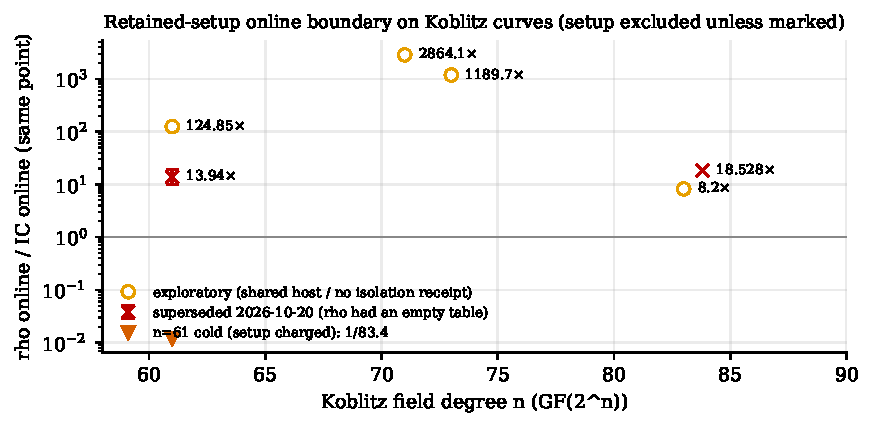
\includegraphics[width=\linewidth]{figures/fig-koblitz-online.pdf}
\caption[]{Rho online time over IC online time on the identical public point,
reusable IC preparation excluded. Open circles: exploratory (verified
answers, no qualifying isolation receipt; three repeats of one point or a
single point). Filled square: the admitted 64-workload panel with its 95\%
bootstrap interval. Triangle: the same $n=61$ candidate with set-up
charged (cold). Sources: \art{docs/ic/boundary_targets.json},
\art{docs/ic/PLAN_IC_ACCOUNTING_FIXES_20261007.md},
\art{research/n83_dense_root_20261013/}.}
\label{fig:online}
\end{figure}

The exploratory ratios are large and irregular because a one-point online
window measures the luck of one relation search against one rho walk; the
admitted panel's range over 64 workloads is $1.06$--$648.6\times$. The
admitted point is a constant-factor online result at $n=61$ (47-bit
subgroup) with preparation retained; it is not a cold result, not a
scaling law, and not an asymptotic claim.

\emph{Retired as an index-calculus win (14 October).} Every rung of this
ladder compares index calculus with a retained table against rho with
none. Given a distinguished-point table of equal or smaller size,
Bernstein--Lange preprocessing rho~\cite{bl2012} is $53$--$317\times$
faster online than the compact-orbit arm on the same 64 targets at $n=41$,
53 and 61 (\S\ref{sec:ladder}). At $n=83$ (\S\ref{sec:n83}) rho with a
table matched to the index calculus's set-up time or memory won every pair
that was run. The ladder therefore measures what a table buys, and generic
rho buys more per byte. The validation sweep later found
\art{docs/ic/BOUNDARY_TARGETS.md} still printing the $13.94\times$ as a
win; it is superseded
(\art{research/validation_sweep_20261019/B-benchmarks/VERDICT_TABLE.md}).

\subsection{The $n=83$ campaign}\label{sec:n83}

Degree 83 was the programme's largest Koblitz target with a working
pipeline: 145 study directories between 4 and 21 October
(Appendix~\ref{sec:catalogue}, clusters beginning ``n83'' and ``f6-n83'').
In order:
\begin{itemize}
\item \emph{F6 micro-studies, 4--5 October} (24 directories, almost all on
  the $a=0$ curve). They kept kernel gains (queries up to $2.998\times$
  faster, resident memory $-52\%$) and shrank SAT encodings, but every
  ordinary solve timed out; four-summand coverage was at most
  $4.662\cdot10^{-12}$ of the subgroup and no natural relation was found.
  On the 81-bit $a=0$ gate curve, SAT and XCNF decompositions succeed only
  with a known witness, and the prebuilt-base question is an open problem
  record.
\item \emph{The $a=1$ point, 7--12 October.} The archived K600 point read
  $8.2\times$ online and was re-measured slower (above).
\item \emph{Root-index capacity, 13--16 October} (25 directories). Root-index
  layouts grew the $a=1$ base from K512 ($84{,}992$ points) to K3596
  ($596{,}936$ points) within 14\,GiB. The dense root index cut probes per
  relation from $300{,}021.9$ to $169{,}069.8$ (K1500 to K1798; paired
  difference $130{,}952$ $[52{,}058,209{,}990]$), a within-IC result that
  stands; its one-point online $18.528\times$ is retired
  (\art{research/n83_dense_root_20261013/}).
\item \emph{Factor-base selection, 14--16 October} (56 directories). Root4,
  root11 and root21 layouts, Bloom filters, sparse and canonical variants
  and $K$ screens from 100 to 20{,}000 points selected within index calculus;
  the best means are about 26--29\,ms online (K3425, K3450, K3500), and
  many screens end \textsc{bounded\_unknown}. A three-hash 512\,MiB Bloom
  filter cut a K3300 online mean from $34.77$ to $31.32$\,ms
  (\art{research/n83_root11_bloom_results_20261015/}); a K3350 win of
  $7.18\%$ did not replicate.
\item \emph{Tier-1 online readings, 14--16 October} (14 directories): median
  rho/IC of $54.1$, $210.3$, $113.0$, $104.2$, $35.1$, $413.3$ (one point)
  and $208.7\times$ (K3072, five fresh points, $[38.3,2{,}510]$;
  \art{research/n83_tier1_online_20261016/}), all against a rho with no
  table and with set-up excluded.
\item \emph{The control, 16 October.} Bernstein--Lange rho given a
  distinguished-point table matched to the index calculus's set-up time or
  memory was faster online in every pair run: IC/rho $3.74$
  $[2.65,11.05]$ (K3300, time-matched), $40.61$ (K3300, memory-matched),
  and $81.5$--$395.5$ (K600)
  (\art{research/20261016-n83-precomputed-rho-control/}). Only the K3300 and
  K600 bases were paired; the K3072 reading was not, so its retirement rests
  on the same mechanism rather than on its own measurement. The validation
  sweep and the ledger audit retired all the online readings on 19--20
  October.
\item \emph{Cold, 16--21 October} (11 directories). The cold one-target
  process fell from about 150\,s (K1024) to $119.8$\,s (K1120, holdout) and
  $113.8$\,s (K1107; \art{research/n83_cold_base_confirm_20261021/}), against
  a rho online time of about 2.2--2.6\,s on the same hosts. No matched cold
  rho was run, so no cold ratio is admitted; the hosted single-target
  benchmark's $133.7\times$ is the nearest cold figure
  (\art{benchmarks/20261014-n71-n83-hosted-single-target/}).
\end{itemize}
The open pull requests at the time of writing include further $n=83$ work
($m=4$ queries on a retained 16{,}627-column base, AWS replays, shared-binary
panels); none is on \texttt{main} (Appendix~\ref{sec:openprs}).

\subsection{Leaderboard Table A: the Koblitz rules}\label{sec:tablea}

Table~A of \art{docs/ic/LEADERBOARD.md} prices one unseen public target on
Koblitz curves at $n=41$--$61$ ($\log_2r=36.6$--$47.2$), cold, against rho on
the same point. Its history is a sequence of rules, each a pipeline baseline
plus a rho reference (\art{research/ic_tool_program/}):
\begin{itemize}
\item \emph{Rule v3}: IC/rho $5.23$--$21\times$, the figure still printed
  in Table~A, which remains unvalidated (pre-gate).
\item \emph{Baselines v4--v8} (16--17 October): head-of-main, scan-key
  (v5, $1.20$--$1.24\times$ cold), scan-fold (v6, $1.33$--$1.40\times$),
  build streams (v7, $1.07$--$1.13\times$) and admitted prefetch (v8,
  $1.06\times$), together $1.90$--$1.98\times$ cheaper cold than v4
  (\art{benchmarks/20261017-ic-r12-admitted-prefetch/}). Seven further
  candidates (prefetch gates, filter slots, huge pages, a wider base) did
  not clear their rounds.
\item \emph{Rules v6, v7}: cold rho still faster at every size,
  $3.78$--$12.06\times$ and then $3.43$--$11.51\times$; but their rho
  references ran at $0.57$--$0.85$ of the strong walk per step, so the
  distance was understated (\art{benchmarks/20261016-ic-rule-v7/}).
\item \emph{Rule v8} (19 October): with a matched GFNI rho the cold distance
  is $4.67$ $[4.34,5.07]$ to $18.07$ $[15.98,20.58]\times$, $1.30$--$1.58\times$
  the v7 control, with a fitted slope of $0.168$ per $\ln r$
  (\art{benchmarks/20261019-ic-matched-rho-v8/}). The run is archived as
  incomplete although its row is listed.
\item \emph{Rule v4 recipe} (24 October; \S\ref{sec:ladder3}): a paired
  retuning improved one size of six; with rho priced in the same process at
  the canonical batched step the distance is $9.9$--$43\times$. Its
  validation file is withheld because its rho reference may not be the
  strongest, so it is not an admitted row either.
\end{itemize}
Table~C prices a 32-target batch on nine Koblitz curves ($\log_2 r=18$--$47.2$)
against batch rho on the same targets: $3.62$--$14.9\times$, a historical
diagnostic under the one-target rule. All nine failed the 24 October
validation gate, and Table~D, the Joux--Vitse historical study, is withheld.

The validation sweep found that Table~A understates its gap to rho by
$1.7$--$2.0\times$, and the 24 October validation gate did not check Table~A
(\art{research/ic_validation_gate_20261024/}). Rules v8 and v4 measure the
same sizes against differently built rho references and are kept apart
(Definition~\ref{def:domain}).

\subsection{ECC2K-130}\label{sec:ecc2k130}

ECC2K-130 is the $a=0$, $n=131$ member of the same family, with a 130-bit
prime subgroup and rho at about $2^{60.81}$ group operations. The compact
producer already solves $n=41,53,61,71,73$ of the family; about 300 notes
under \art{research/notes/ecc2k130/} price the routes to $n=131$ itself. No
route prices below rho.
\begin{itemize}
\item \emph{Extrapolating the producer.} The fitted probes-per-relation law
  $C\,r/(n^2K^2)$ with $C=1$ gives $1.1\cdot10^{18}$ core-years at $K=600$
  and $6.8\cdot10^{8}$ at $K=10^{12}$ columns
  (\art{RESEARCH_ECC2K130_IC_FEASIBILITY.md}, with the unexplained
  factor-of-5 gap in $C$ of \S\ref{sec:corrections}).
\item \emph{Decomposition oracles.} Decompositions exist, but no oracle
  finds one for less than $2^{131}$ per family; using unions of Frobenius
  orbits lowers the family's bottom from $2^{132.58}$ to $2^{124.99}$, still
  $2^{64.18}$ times rho, and needs a materialised base of $2^{44.53}$ points
  at $m=3$
  (\art{research/notes/ecc2k130/RESEARCH_ECC2K130_DECOMPOSITION_TARGETS.md}).
  Relation sweeps over $m$ give a best single-relation row of $+4.98$ bits
  at $m=4$ (with $2^{70.79}$ bytes) and a best honest $m=8$ row of $+13.59$
  bits with the Frobenius quotient
  (\art{research/notes/ecc2k130/RESEARCH_ECC2K130_RELATION_SWEEPS.md}).
  Crossbred, RR-solver and WDSat oracles are engineering only: Crossbred is
  $0.023$ of F4's bit operations at $m=3$ but slower end to end, and the RR
  solvers' advantage over Semaev at $d=6$ is worthless against brute force.
\item \emph{Linearisation.} Plain linearisation leaves a gap of $70.19-b_{\max}$
  bits to rho; the best bilinear XL setting, with each Macaulay solve
  charged, is $71.82$ bits at $\omega=2$ ($78.15$ at $\omega=2.81$), and a
  trilinear variant is worse ($87.16$ bits)
  (\art{research/linearization_reach_20260930/},
  \art{research/xl_bilinear_core_20261006/},
  \art{research/xl_trilinear_t_unknown_20261006/}).
\item \emph{Weil descent.} The descent-degree note's rows are $m=3$ with a
  free oracle at $2^{68.58}$; $m=4$ at degree 4, $2^{68.43}$ ($+7.62$ bits,
  now contradicted); and $m=4$ at degree 5, $2^{71.13}$ ($+10.32$) at $w=1$ and
  $2^{106.52}$ ($+45.71$) at $w=2$, in unconverted column touches
  (\art{research/notes/ecc2k130/RESEARCH_ECC2K130_DESCENT_DEGREE.md}).
  The studies behind these rows, and the hybrid guess that puts the $m=4$
  row at $+8.43$ to $+58.27$ bits, are in \S\ref{sec:binary-descent}.
\item \emph{Covers.} After the magic-number correction, a genus-130
  hyperelliptic curve would cost $2^{37.17}$, but no such cover exists; the
  $N=130$ counterfactual is genus 255 at a modelled $2^{55.60}$ against rho's
  $2^{60.31}$, and measuring one relation trial turns that margin negative
  (\S\ref{sec:ladder3}). The best explicit curve construction reaches genus
  $2^{28.92}$
  (\art{research/notes/ecc2k130/RESEARCH_ECC2K130_CURVE_CONSTRUCTION.md}).
  The isogeny class has 262 curves of conductor gap 263 and no measured
  level effect (\S\ref{sec:transfer}); rho on the degree-263 leaves keeps
  only the negation map, an $11.45\times$ penalty
  (\art{research/notes/ecc2k130/isogeny_rho_speed_20260930/}).
\item \emph{Rho itself.} The separate GPU rho estimate is about 4.3 RTX PRO
  6000 card-years (\art{paper/ecc2k130/}); on one CPU core the ECC2K-130
  client walks 13.2 million steps per second
  (\art{research/certicom131_rho_ic_bench_20261022/}). Signed $\sigma$ steps
  cut modelled GPU time to $0.961$--$0.970$
  (\art{benchmarks/20261014-ecc2k130-signed-sigma/}).
\end{itemize}
Index calculus is not a route to ECC2K-130 on this evidence; every priced
route is at least about 5 bits above rho (the $m=4$ single-relation row, at
$2^{70.79}$ bytes), and most are tens of bits.

\subsection{Factor bases closed under $\ZZ[\tau]$}

The $\ZZ[\tau]$ small-norm multiplier base of 23 October
(\art{research/ic_improve_20261023/README.md}) is the latest Koblitz
change: $1.9$--$4.4\times$ child CPU at $n=41$--$61$ and $6.2$--$10.5\times$
at $n=71$, against the programme's own producer, exponent unchanged; it is
discussed with the other known-logarithm bases in \S\ref{sec:ladder3}.
